%%%
% Plantilla de Memoria
% Modificación de una plantilla de Latex de Nicolas Diaz para adaptarla 
% al castellano y a las necesidades de escribir informática y matemáticas.
%
% Editada por: Mario Román
%
% License:
% CC BY-NC-SA 3.0 (http://creativecommons.org/licenses/by-nc-sa/3.0/)
%%%

%%%%%%%%%%%%%%%%%%%%%%%%%%%%%%%%%%%%%%%%%
% Thin Sectioned Essay
% LaTeX Template
% Version 1.0 (3/8/13)
%
% This template has been downloaded from:
% http://www.LaTeXTemplates.com
%
% Original Author:
% Nicolas Diaz (nsdiaz@uc.cl) with extensive modifications by:
% Vel (vel@latextemplates.com)
%
% License:
% CC BY-NC-SA 3.0 (http://creativecommons.org/licenses/by-nc-sa/3.0/)
%
%%%%%%%%%%%%%%%%%%%%%%%%%%%%%%%%%%%%%%%%%

%----------------------------------------------------------------------------------------
%	PAQUETES Y CONFIGURACIÓN DEL DOCUMENTO
%----------------------------------------------------------------------------------------
%%% Configuración del papel.
% microtype: Tipografía.
% mathpazo: Usa la fuente Palatino.
\documentclass[a4paper, 11pt]{article}
\usepackage[protrusion=true,expansion=true]{microtype}
\usepackage{mathpazo}


% Indentación de párrafos para Palatino
\setlength{\parindent}{0pt}
  \parskip=8pt
\linespread{1.05} % Change line spacing here, Palatino benefits from a slight increase by default


%%% Castellano.
% noquoting: Permite uso de comillas no españolas.
% lcroman: Permite la enumeración con numerales romanos en minúscula.
% fontenc: Usa la fuente completa para que pueda copiarse correctamente del pdf.
\usepackage[spanish,es-noquoting,es-lcroman]{babel}
\usepackage[utf8]{inputenc}
\usepackage[T1]{fontenc}
\selectlanguage{spanish}


%%% Gráficos
\usepackage{graphicx} % Required for including pictures
\usepackage{wrapfig} % Allows in-line images
\usepackage[usenames,dvipsnames]{color} % Coloring code

%%% Matemáticas
\usepackage{amsmath}


%%% Bibliografía
\makeatletter
\renewcommand\@biblabel[1]{\textbf{#1.}} % Change the square brackets for each bibliography item from '[1]' to '1.'
\renewcommand{\@listI}{\itemsep=0pt} % Reduce the space between items in the itemize and enumerate environments and the bibliography
\usepackage{hyperref}
\hypersetup{
	colorlinks   = true,    % Colours links instead of ugly boxes
	urlcolor     = red,    % Colour for external hyperlinks
	linkcolor    = red,    % Colour of internal links
	citecolor    = blue      % Colour of citations
}

\usepackage{tikz}
\usetikzlibrary{mindmap,trees}

%%% CÓDIGO

\usepackage{listings}   
\usepackage{xcolor}
\lstdefinestyle{customc}{	
	backgroundcolor=\color{white},    % choose the background color; you must add \usepackage{color} or \usepackage{xcolor}; should come as last argument
	basicstyle=\footnotesize\ttfamily,% the size of the fonts that are used for the code
	breakatwhitespace=false,          % sets if automatic breaks should only happen at whitespace
	breaklines=true,                  % sets automatic line breaking
	captionpos=b,                     % sets the caption-position to bottom
    commentstyle=\itshape\color{purple!40!black},     % comment style
	deletekeywords={...},             % if you want to delete keywords from the given language
	escapeinside={\%*}{*)},           % if you want to add LaTeX within your code
	extendedchars=true,               % lets you use non-ASCII characters; for 8-bits encodings only, does not work with UTF-8
	frame=single,	                  % adds a frame around the code
	keepspaces=true,                  % keeps spaces in text, useful for keeping indentation of code (possibly needs columns=flexible)
	keywordstyle=\bfseries\color{green!40!black},       % keyword style
	language=C,                       % the language of the code
	morekeywords={*,...},             % if you want to add more keywords to the set
	numbers=left,                     % where to put the line-numbers; possible values are (none, left, right)
	numbersep=5pt,                    % how far the line-numbers are from the code
	numberstyle=\tiny\color{gray},    % the style that is used for the line-numbers
	rulecolor=\color{black},          % if not set, the frame-color may be changed on line-breaks within not-black text (e.g. comments (green here))
	showspaces=false,                 % show spaces everywhere adding particular underscores; it overrides 'showstringspaces'
	showstringspaces=false,           % underline spaces within strings only
	showtabs=false,                   % show tabs within strings adding particular underscores
	stepnumber=2,                     % the step between two line-numbers. If it's 1, each line will be numbered
    stringstyle=\color{orange},       % string literal style
	tabsize=2,	                      % sets default tabsize to 2 spaces
	title=\lstname,                   % show the filename of files included with \lstinputlisting; also try caption instead of title
	identifierstyle=\color{blue}
}

\lstdefinestyle{customasm}{
	belowcaptionskip=1\baselineskip,
	frame=L,
	xleftmargin=\parindent,
	language=[x86masm]Assembler,
	basicstyle=\footnotesize\ttfamily,
	commentstyle=\itshape\color{purple!40!black},
}

\DeclareFixedFont{\ttb}{T1}{txtt}{bx}{n}{8} % for bold
\DeclareFixedFont{\ttm}{T1}{txtt}{m}{n}{8}  % for normal


\lstdefinestyle{customPY}{
	language=Python,
	basicstyle=\ttm,
	otherkeywords={self},             % Add keywords here
	keywordstyle=\ttb\color{blue},
	emph={MyClass,__init__},          % Custom highlighting
	emphstyle=\ttb\color{red},    % Custom highlighting style
	stringstyle=\color{orange},
	frame=tb,                         % Any extra options here
	showstringspaces=false       
}

\lstset{escapechar=@,style=customc}


%% cosas 

\usepackage[margin=1in]{geometry}

\usepackage{times}


%----------------------------------------------------------------------------------------
%	TÍTULO
%----------------------------------------------------------------------------------------
% Configuraciones para el título.
% El título no debe editarse aquí.
\renewcommand{\maketitle}{
  \begin{flushright} % Right align
  
  {\LARGE\@title} % Increase the font size of the title
  
  \vspace{50pt} % Some vertical space between the title and author name
  
  {\large\@author} % Author name
  \\\@date % Date
  \vspace{40pt} % Some vertical space between the author block and abstract
  \end{flushright}
}

%% Título
\title{\textbf{Construyendo sobre Prelude}\\ % Title
					una introducción a Emacs.} % Subtitle

\author{\textsc{Francisco Navarro Morales} % Author
\\{\textit{GRG121}}} % Institution

\date{\today} % Date





%----------------------------------------------------------------------------------------
%	DOCUMENTO
%----------------------------------------------------------------------------------------

\begin{document}
	
	
	\begin{titlepage}
		\begin{center}
			\vspace*{2cm}
			
			{\Huge \textbf{Obtención de la fórmula maestra.}}
			
			 ALGORITMICA 
			
			
			\vspace{0.5cm}
			
			
		    \centering 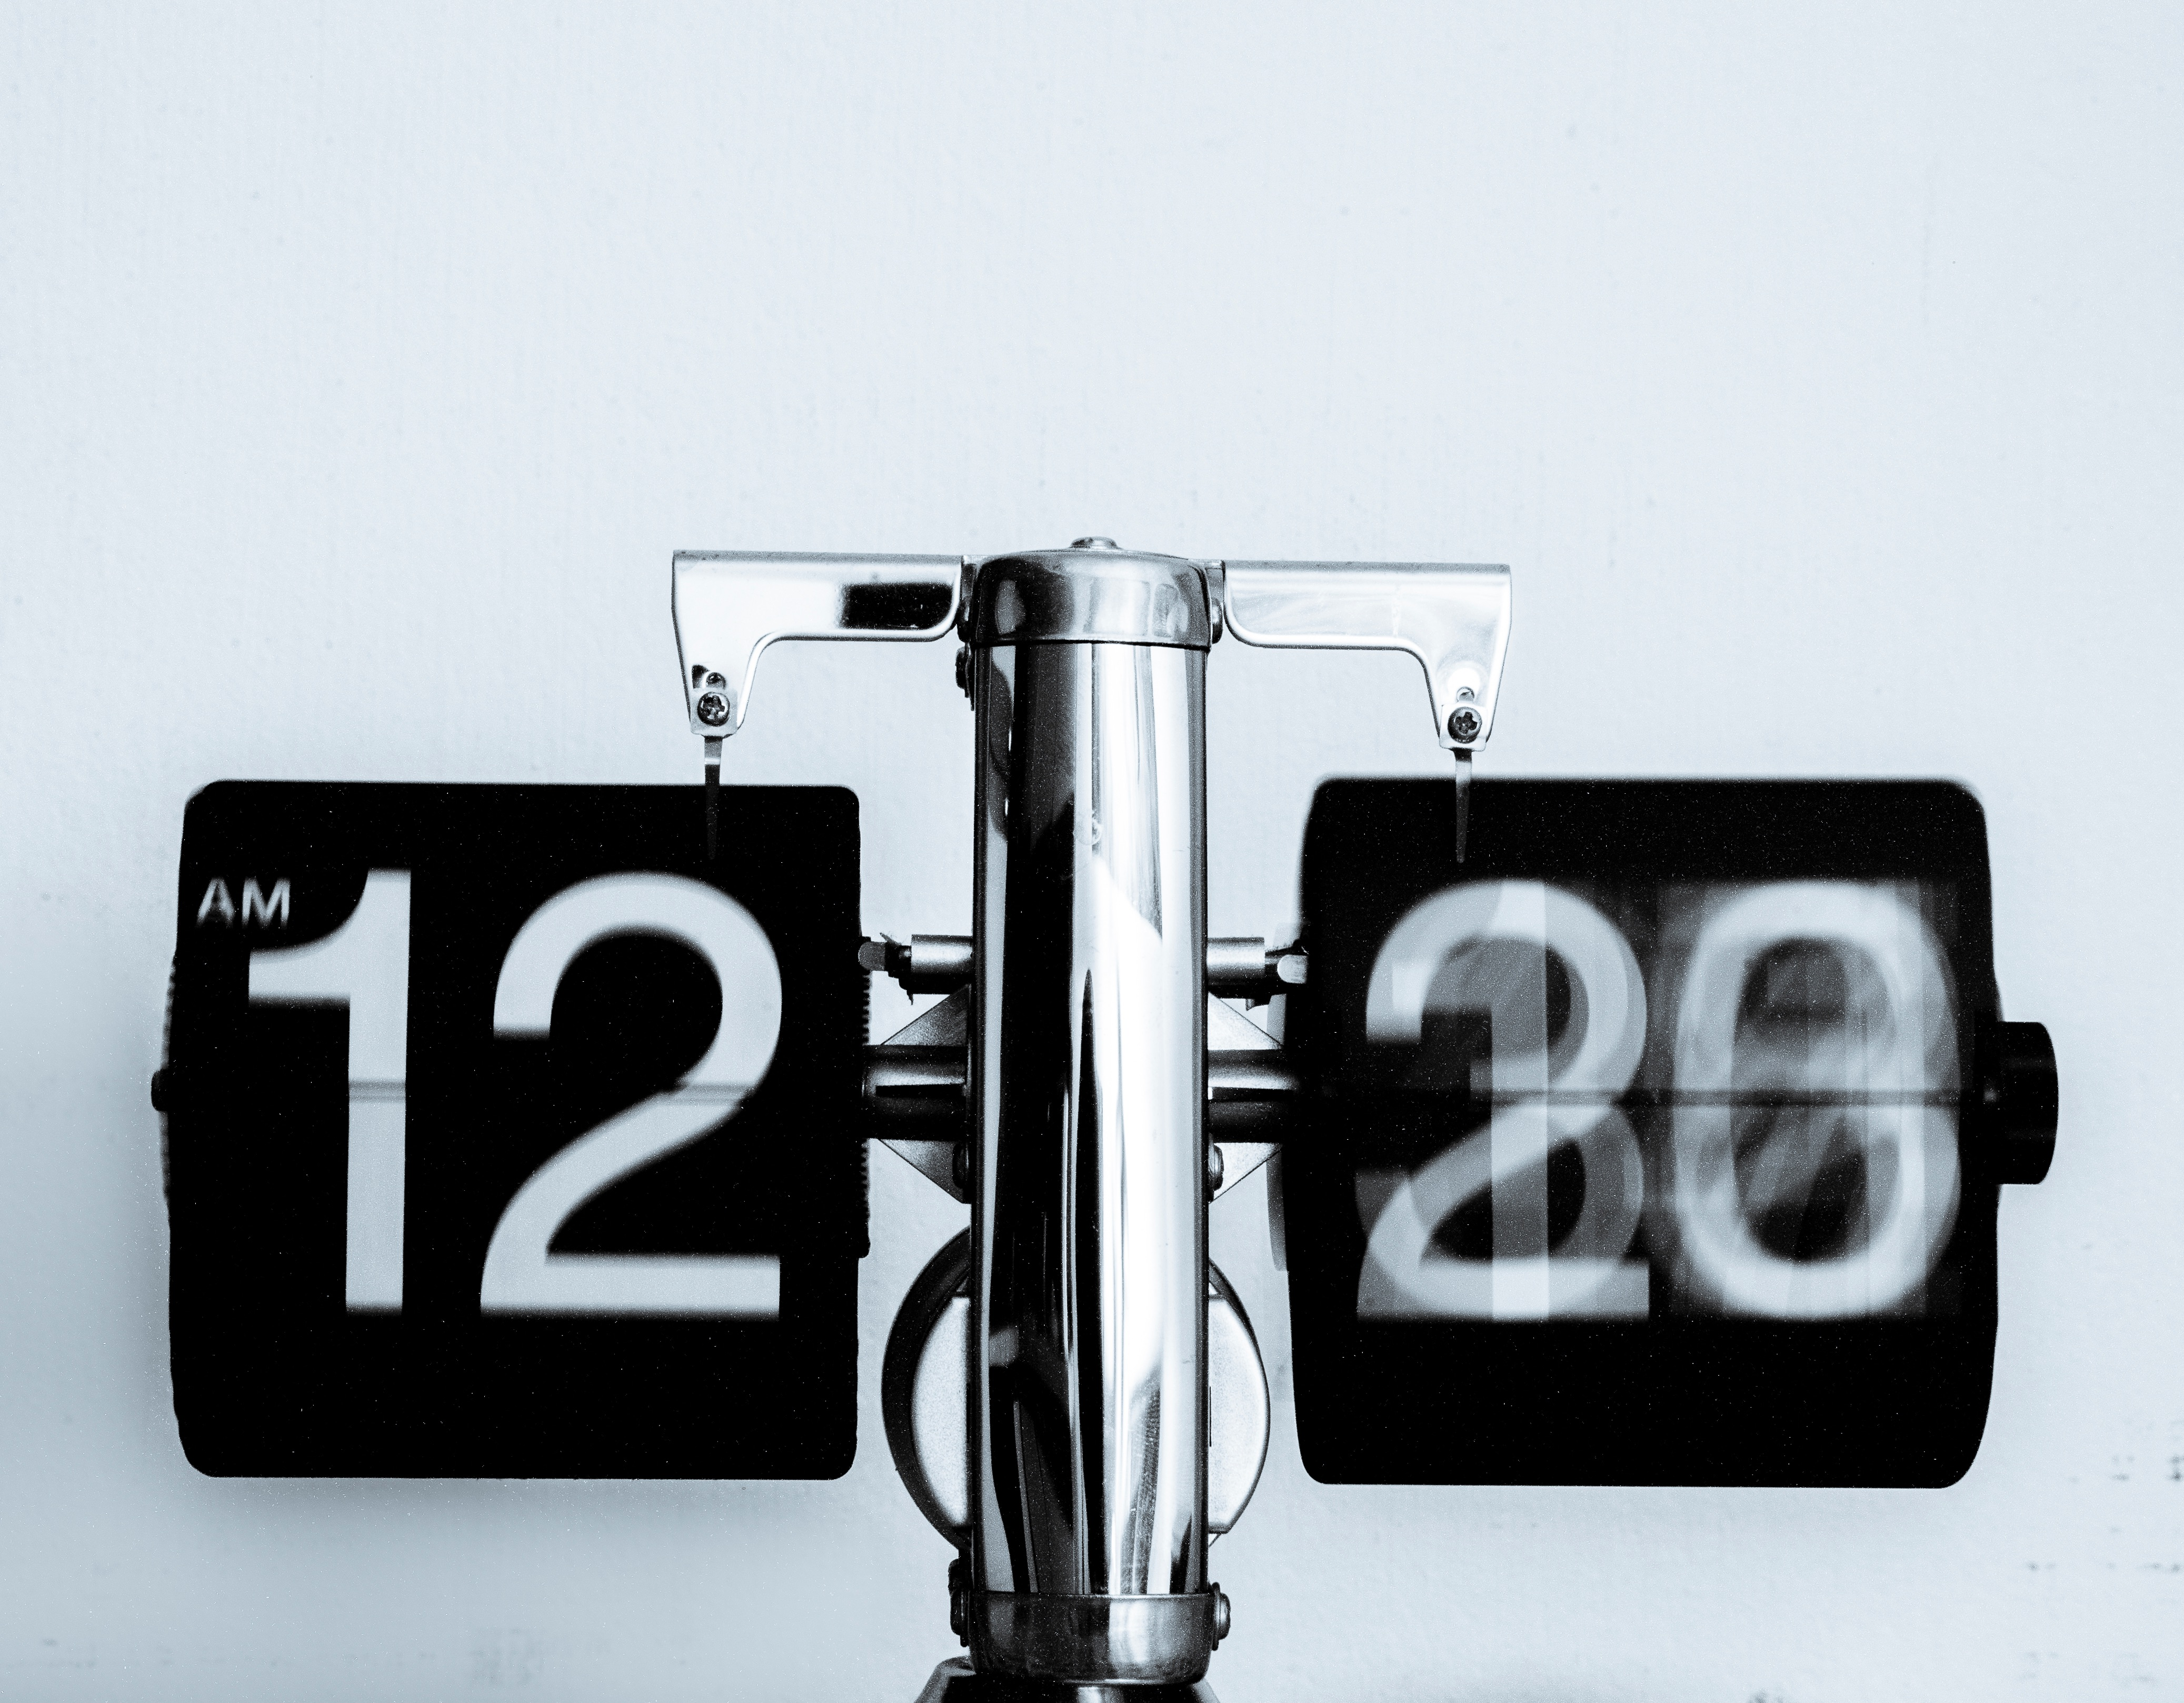
\includegraphics[width=0.7\textwidth]{cover.jpg}
		  
			
			\vspace{2cm}
			
			\textbf{Francisco Navarro Morales - GRG121 }
			
			\vfill
			
			Segundo curso del Grado de Ingeniería Informática\\
			Universidad de Granada\\
			curso 2016-2017\\
			
		\end{center}
	\end{titlepage}


%\maketitle % Print the title section

%% Resumen (Descomentar para usarlo)
\renewcommand{\abstractname}{Resumen} % Uncomment to change the name of the abstract to something else
%\begin{abstract}
% Resumen aquí
%\end{abstract}

%% Palabras clave
%\hspace*{3,6mm}\textit{Keywords:} lorem , ipsum , dolor , sit amet , lectus % Keywords
%\vspace{30pt} % Some vertical space between the abstract and first section


%% Índice
%%{\parskip=2pt
%%  \tableofcontents
%%}

%%% Inicio del documento

\pagebreak
En general, cuando utilizamos la metodología de \textbf{divide y vencerás}, nos encontramos con $a$ llamadas recursivas de tamaño $n/b$ para las cuales necesitamos un tiempo $f(n)=d \times n^p \in O(N^P)$ para la división y combinación de los subproblemas. 

$$t(n)=a t(n/b) + d n^p$$ que con el cambio $n=b^k\rightarrow k= \log_bn$ da lugar a:
$$t(b^k)=at(b^{k-1})+db^{p^k} \rightarrow t_k-at_{k-1}=db^{p^k} \rightarrow x-a = db^{p^k}$$

Se trata de una ecuación lineal no homogénea. El polinomio característico de la parte homogénea es $x-a$, y de la parte no homogénea obtenemos $x-b^p$ 

\begin{itemize}
	\item Si $a=b^p$ entonces tenemos una única raíz de multiplicidad 2: $pc=(x-a)^2$ luego la solución general sería: 
	$$ t(k) = c_1 b^{p^k} + c_2 k b^{p^k} \rightarrow t(n) = c_1b^{log_bn^p}+c_2log_bn \times n^p $$ es decir:
	$$ t(n) = c_1n^p + c_2log_bn \times n^p$$
	
	Como estamos hablando de problemas de eficiencia de algoritmos, es imposible que los coeficientes $c_1$ o $c_2$ sean negativos, por lo que podemos afirmar que, en este caso $t(n)\in O(n^plog_bn)$ 
	\item Si $a>b^p$ entonces tenemos dos raíces distintas de multiplicidad 1: $pc=(x-a)(x-b^p)$ 
	$$t(k)= c_1a^k + c_2b^{p^k} $$ donde $a^k > b^{p^k} $ porque $a>b^p$ luego:
	$$t(n) = c_1a^{log_bn}+c_2b^{{log_bn}^p}==c_1a^{log_bn}+c_2n^p$$
	Se puede demostrar que $a^{log_bn}=n^{log_ba}$ porque, tomando el $log_b$ de ambas partes nos queda: $log_bn \times log_ba = log_ba \times log_bn$ Luego:
	$$t(n)=c_1n^{log_ba}+c_2n^p$$ y como hemos dicho que $c_1n^{log_ba} > c_2n^p$ entonces $$t(b) \in O(n^{\log_ba})$$
	\item Si $a<b^p$ tenemos el mismo resultado que en el caso anterior: 
	$$t(n)=c_1n^{log_ba}+c_2n^p$$ Pero en este caso, $c_1n^{log_ba} < c_2n^p$ y por lo tanto, $$t(b) \in O(n^p)$$
	
\end{itemize}



\end{document}